%
% teil1.tex -- Beispiel-File für das Paper
%
% (c) 2020 Prof Dr Andreas Müller, Hochschule Rapperswil
%
% !TEX root = ../../buch.tex
% !TEX encoding = UTF-8
%
\section{Kirchhoff's Gesetz
\label{circuit:section:teil1}}
\rhead{Problemstellung}
Bevor wir die Laplace Gleichung mithilfe der Lagrange-Funktion herleiten, versuchen wir das auf konventionelle weise indem wir  das Kirchhoffische Gesetz benutzen. 

Das Kirchhoffische Stromgesetz postuliert, dass die Summe der in einen Knoten einfließenden Ströme gleich der Summe der aus diesem Knoten ausfließenden Ströme in einer Schaltung ist. Dies impliziert, dass es in einem Gleichstromkreis im stationären Zustand keine Ladungsakkumulation an irgendeinem Punkt geben kann. Wir betrachten nun einen dreidimensionalen Schaltkreis, in dem die Leitfähigkeit $\sigma$ im gesamten Bereich von Interesse konstant ist. Die Verallgemeinerung des Kirchhoffischen Stromgesetzes im dreidimensionalen Fall besagt, dass die Divergenz der Stromdichte $\vec{J}$ gleich Null ist, es kann kein Strom aus dem Nichts erzeugt werden. Daher gilt \autoref{circuit:current_density_1}.
\begin{equation}
	\nabla \cdot  \vec{J}=0
	\label{circuit:current_density_1}
\end{equation}

Um die Laplace Gleichung auf herkömmliche weise zu finden brauche wir noch ein paar andere Erkenntnisse die hier aufgezeigt werden. Die Stromdichte wird durch \autoref{circuit:current_density_3}definiert. Diese Gleichung besagt, dass die Stromdichte das Verhältnis des Stroms ($I$) zur Flächen ($A$) ist. 
\begin{equation}
\vec{J}=\frac{\vec{I}}{A}
	\label{circuit:current_density_3}
\end{equation}
Wenn das elektrische Feld durch $\vec{E}$ repräsentiert wird und wir ein ohmsches Material vorliegen haben, kann die Stromdichte als Produkt aus Leitfähigkeit und elektrischem Feld an einem gegebenen Punkt im Raum durch \autoref{circuit:current_density_2} beschrieben werden.
\begin{equation}
\vec{J}=\sigma \vec{E}
\label{circuit:current_density_2}
\end{equation}


Das elektrische Feld kann dabei als negativer Gradient der Potential Funktion $\phi$ geschrieben werden, d.h.
\begin{equation}
\vec{E}=-\nabla \phi
\label{circuit:current_density_4}
\end{equation}

Daher erhalten wir aus den Gleichungen \autoref{circuit:current_density_1}, \autoref{circuit:current_density_2} und \autoref{circuit:current_density_4} \autoref{circuit:current_density_5}.
\begin{equation}
\nabla \cdot (\sigma \nabla \phi)=0
\label{circuit:current_density_5}
\end{equation}

Wenn wir annehmen, dass die Leitfähigkeit im gesamten betrachteten Raum konstant ist, gilt zudem \autoref{circuit:current_density_6} welche die Laplace gleichung darstellt.
\begin{equation}
\nabla^2 \phi=0
\label{circuit:current_density_6}
\end{equation}

\section{Variationsprinizip}
Im nächsten Schritt versuchen wir, \autoref{circuit:current_density_6} mithilfe des Variationsprinzips herzuleiten. Dafür drücken wir die Wärmeerzeugungsrate $P$ in einem von einer Grenze $S$ umgebenen Volumen $V$ durch \autoref{circuit:current_density_7} aus. Aus den Prinzipien der Thermodynamik wissen wir, dass die Entropie in einem geschlossenen System zunimmt. Daher wenden wir das Variationsprinzip auf \autoref{circuit:current_density_7} an und lösen es. Dies sollte uns die minimale Energie in einem zweidimensionalen oder dreidimensionalen Raum geben. Auf den ersten Blick mag \autoref{circuit:current_density_7} nicht sehr intuitiv erscheinen. Daher könnten wir die Gleichung auch anders formulieren, wie in \autoref{circuit:current_density_8} gezeigt, wobei $U^2=\left( \nabla \phi \right)^2$ und $R=\frac{1}{\sigma}$.

\begin{equation}
	P=\frac{U^2}{R}
	\label{circuit:current_density_8}
\end{equation}

\section{Lösen der Lagrange Funktion}
In folgendem Kapitel lösen wir die Lagrange-Funktion mithilfe der Euler Ostrogradsky Differentialgleichung welche auch in \autoref{buch:felder:ostrogradski:eqn:euler-ostrogradski} gefunden werden kann.


\begin{equation}
P=\int_V \sigma(\nabla \phi)^2 d V
\label{circuit:current_density_7}
\end{equation}

Nehmen wir nun \autoref{circuit:current_density_7} und wenden Euler-Ostrogradsky auf die Gleichung an:
\begin{enumerate}
	\item Schritt: Lagrange-Funktion des Problems ohne $\sigma$
	\begin{equation}
		L(x, U, U_x)= U_x^2 = \left(U_{x_1}^2+U_{x_2}^2\right)
	\end{equation}
	\item Schritt: partielle Ableitungen
	\begin{equation}
		\begin{aligned}
			\frac{\partial L}{\partial U}=0\\
			\frac{\partial L}{\partial U_{x_1}}=2U_{x_1}\\
			\frac{\partial L}{\partial U_{x_2}}=2U_{x_2}\\
		\end{aligned}
	\end{equation}
	\item Schritt: Ableiten nach $x_1$ und $x_2$
	\begin{equation}
		\begin{aligned}
			\frac{\partial}{\partial x_1}\frac{\partial L}{\partial U_{x_1}}(x,\phi,\nabla \phi)=2\frac{\partial \phi}{\partial {x_1}}\cdot \frac{\partial}{\partial x_1}\\
			\frac{\partial}{\partial x_2}\frac{\partial L}{\partial U_{x_2}}(x,\phi,\nabla \phi)=2\frac{\partial \phi}{\partial {x_2}} \cdot \frac{\partial}{\partial x_1}\\
		\end{aligned}
	\end{equation}
	\item Schritt: Euler-Ostrogradsky Differentialgleichung
	\begin{equation}
		-\frac{\partial}{\partial x_1}\cdot 2\frac{\partial \phi}{\partial {x_1}}-\frac{\partial}{\partial x_2}\cdot 2\frac{\partial \phi}{\partial {x_2}}=-2\Delta\phi
	\end{equation}
	\item Schritt: Mögliche Lösungen
	\begin{equation}
	\sigma \cdot 2\Delta\phi=0
	\end{equation}
Wir können nun noch durch $2\sigma$ teilen und bekommen die Laplace Gleichung aus \autoref{circuit:current_density_6}. Somit wurde gezeigt dass die Laplace Gleichung auch dem Variationsprinzip gefunden werden kann sowie auch mit den Kirchhoffischen Regeln.
	\begin{equation}
	\Delta\phi=0=\frac{\delta^2\phi}{\delta x^2}+\frac{\delta^2\phi}{\delta y^2}
	\label{circuit:laplace1}
	\end{equation}
	%\begin{equation}
	%	\Delta \phi(x,y)=\frac{\delta^2\phi}{\delta x^2}+\frac{\delta^2\phi}{\delta y^2}=0
	%\end{equation}
\end{enumerate}

\section{Praktische Anwendungen}
In diesem Kapitel schauen wir uns an wie die elliptische Differentialgleichung aus \autoref{circuit:laplace1} numerisch gelöst werden kann und was Sie eigentlich genau bedeutet.

\autoref{circuit:laplace1} kann diskretisiert werden durch die Differenz zweiter Ordnung wie sie in \autoref{circuit:second-order-central} \cite{enwiki:1220817436} gesehen werden kann.
\begin{equation}
	f^{\prime \prime}(x) \approx \frac{\delta_h^2[f](x)}{h^2}=\frac{\frac{f(x+h)-f(x)}{h}-\frac{f(x)-f(x-h)}{h}}{h}=\frac{f(x+h)-2 f(x)+f(x-h)}{h^2}
	\label{circuit:second-order-central}
\end{equation}
Wenn wir das auf unseren Fall anwenden bekommen wir \autoref{circuit:discret_equation}.
\begin{equation}
	\frac{\phi(x_{i+1}, y_j) - 2\phi(x_i, y_j) + \phi(x_{i-1}, y_j)}{(\Delta x)^2} + \frac{\phi(x_i, y_{j+1}) - 2\phi(x_i, y_j) + \phi(x_i, y_{j-1})}{(\Delta y)^2} = 0 
	\label{circuit:discret_equation}
\end{equation}
Nun können wir auf $\phi(x_i, y_j)$ auflösen und bekommen \autoref{circuit:discret_equation2}.

\begin{equation}
	\phi(x_i, y_j) = \frac{1}{4}(\phi(x_{i+1}, y_{j}) + \phi(x_{i-1}, y_{j}) + \phi(x_{i}, y_{j+1}) + \phi(x_{i}, y_{j-1}))
	\label{circuit:discret_equation2}
\end{equation}
Darum ist die Idee nun nacheinander \autoref{circuit:discret_equation3} auszureichen bis $\phi$ konvertiert.
\begin{equation}
	\phi(x_i, y_j) \to \frac{1}{4}(\phi(x_{i+1}, y_{j}) + \phi(x_{i-1}, y_{j}) + \phi(x_{i}, y_{j+1}) + \phi(x_{i}, y_{j-1}))
	\label{circuit:discret_equation3}
\end{equation}
\subsubsection{Python Beispiel}
In diesem Beispiel betrachten wir eine leitende Platte mit einer Leitfähigkeit von $0,001 \, \text{Siemens pro Meter}$ und einer Größe von einem Quadratmeter. Ein spezifischer Bereich der Platte, definiert durch $0,5 < x < 0,7$ und $0,5 < y < 0,7$, wird mit einem Potential von einem Volt belegt, während der Rand der Platte ein Potential von 0 Volt aufweist.
\begin{figure}[h]
	\centering
	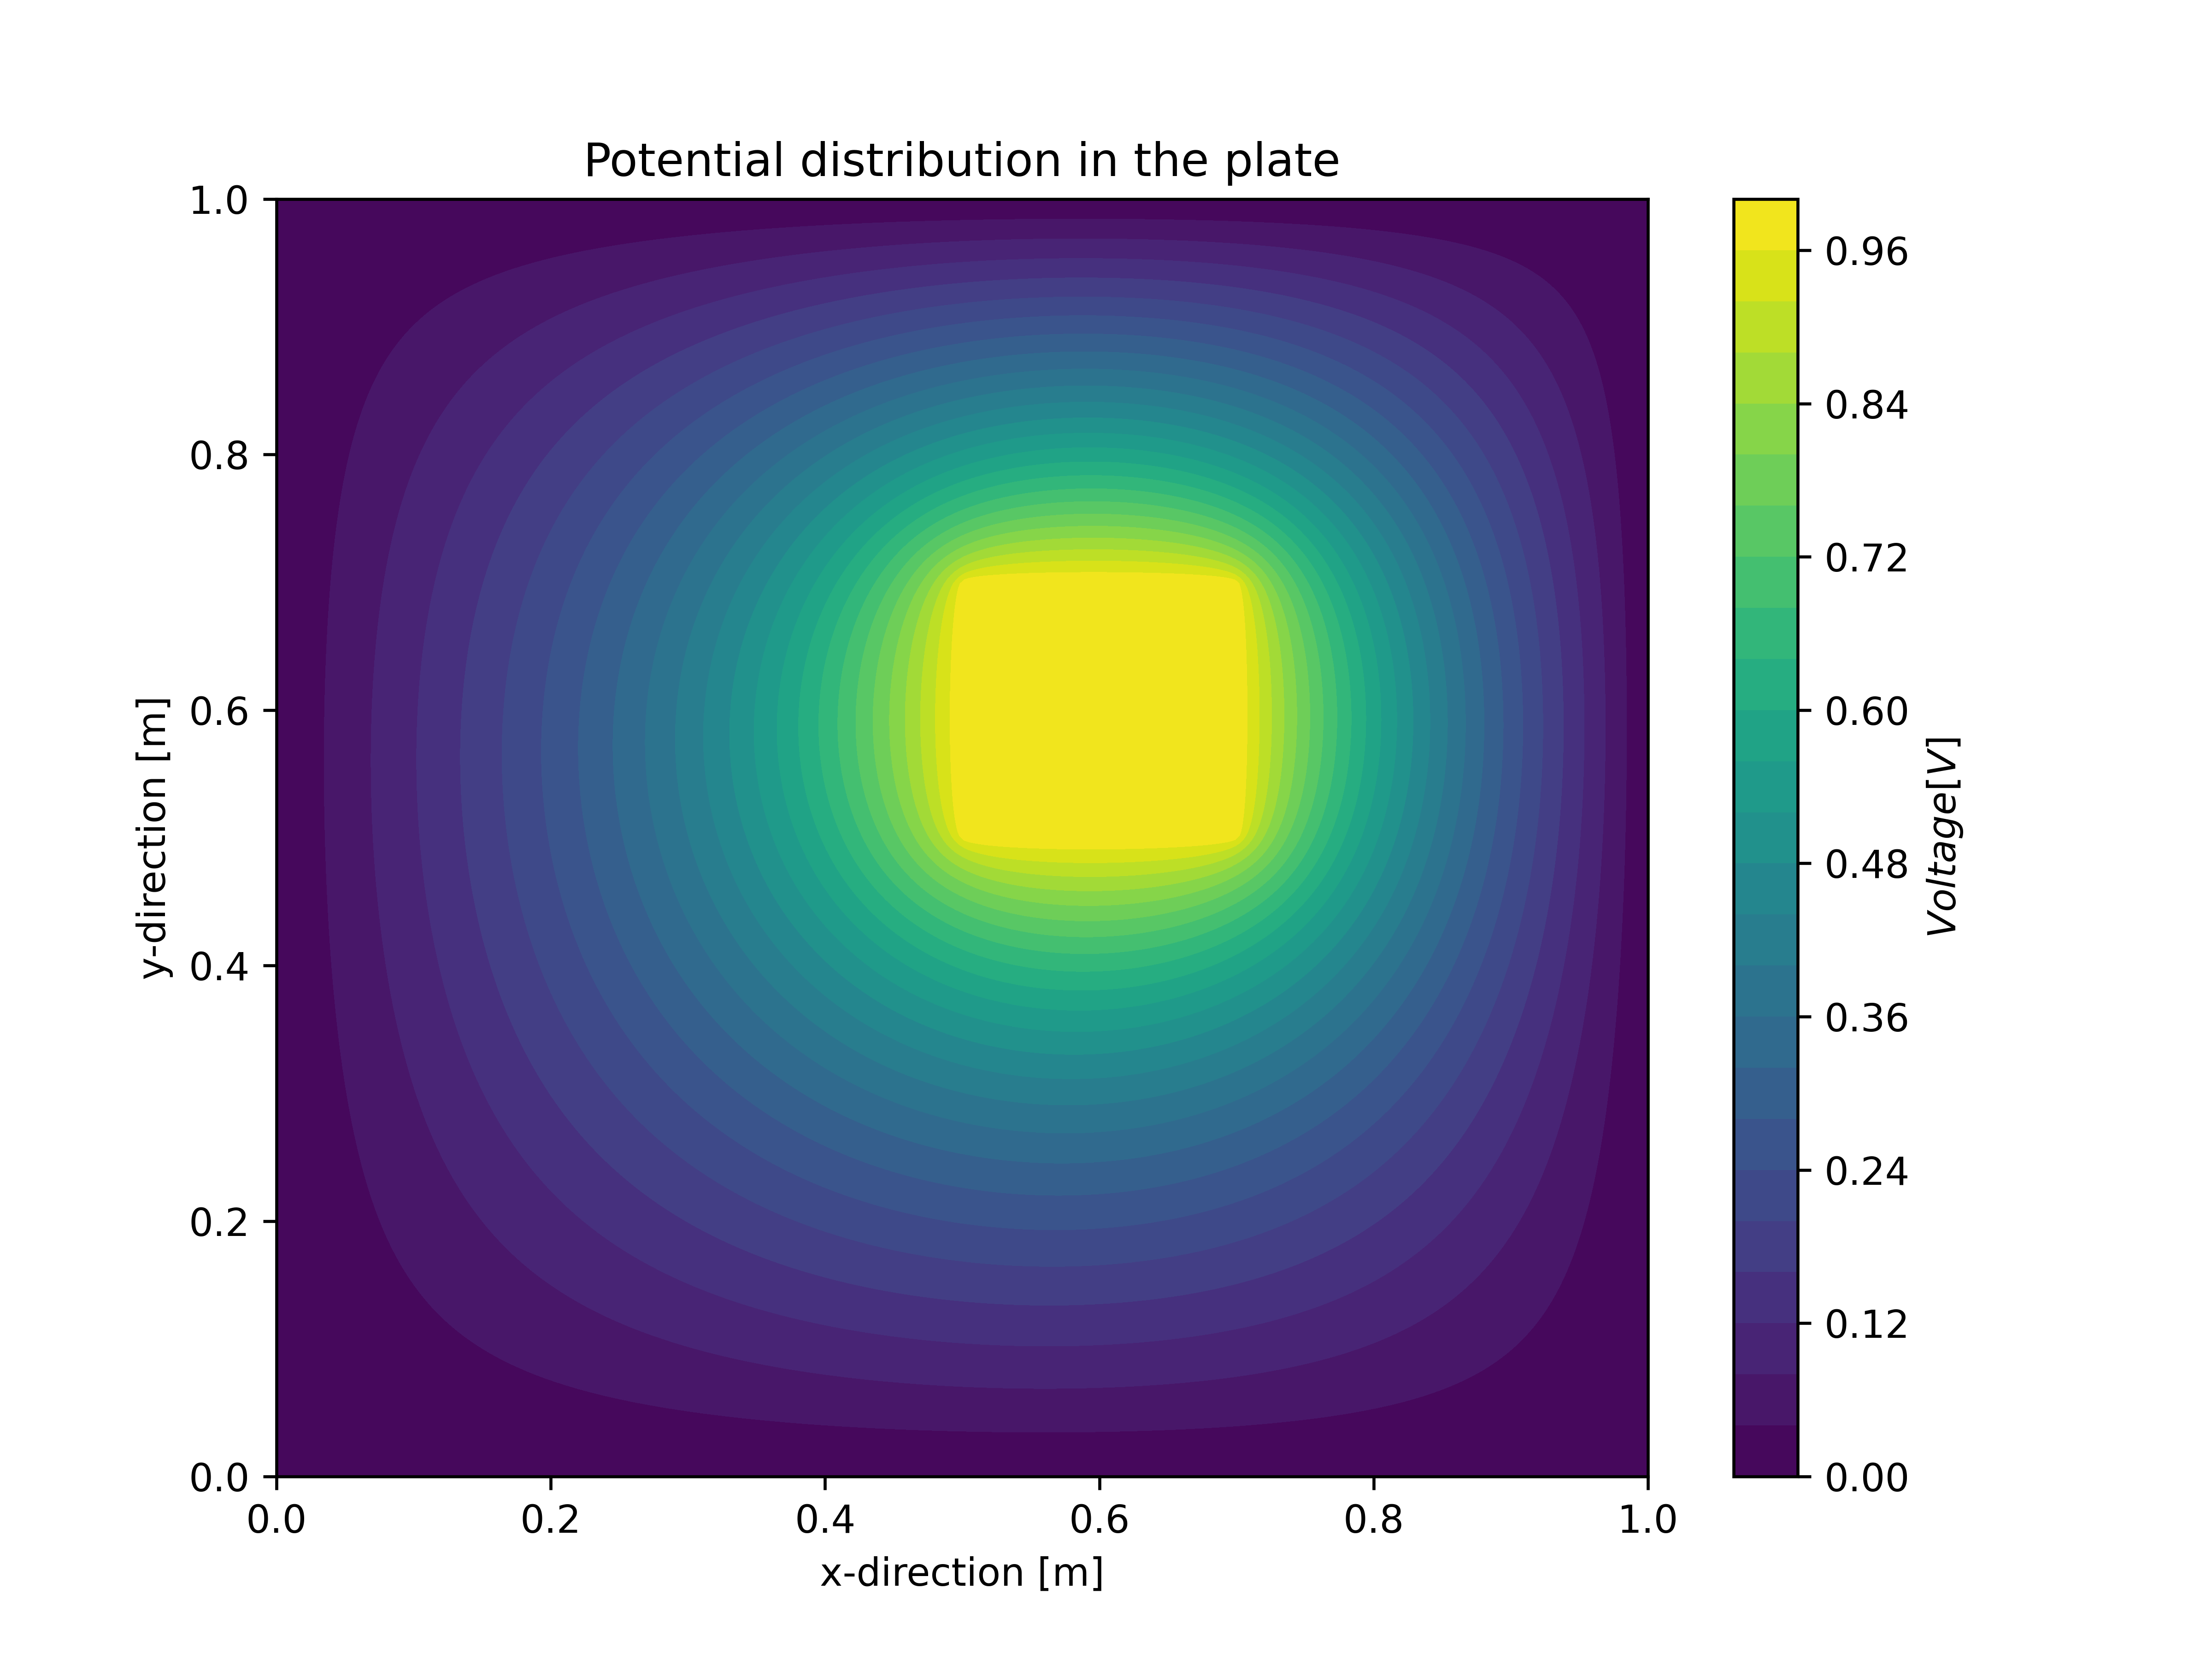
\includegraphics[width=0.99\textwidth]{papers/circuit/potential_distribution.png}
	\caption{Potential Distribution}
	\label{fig:potential_distribution}
\end{figure}
Unter Verwendung von Gleichung \ref{circuit:discret_equation3} zur Berechnung des Potentials erhalten wir die in Abbildung \ref{fig:potential_distribution} dargestellte Potentialverteilung. Dies ermöglicht es uns, das gesamte Potential auf der Platte zu bestimmen.

Sobald das Potential bekannt ist, können wir mithilfe des Gradienten und Gleichung \ref{circuit:current_density_7} die Leistungsdichte an jedem einzelnen Punkt berechnen. Dies führt zu den in Abbildung \ref{fig:power_2d} und \ref{fig:power_3d} dargestellten Leistungsdichteverteilungen, die auch im Beispielskript unter \glqq{}\textbackslash buch\textbackslash papers\textbackslash circuit\textbackslash Präsentation.ipynb\grqq{}  zu finden sind.
\begin{figure}[h]
	\centering
	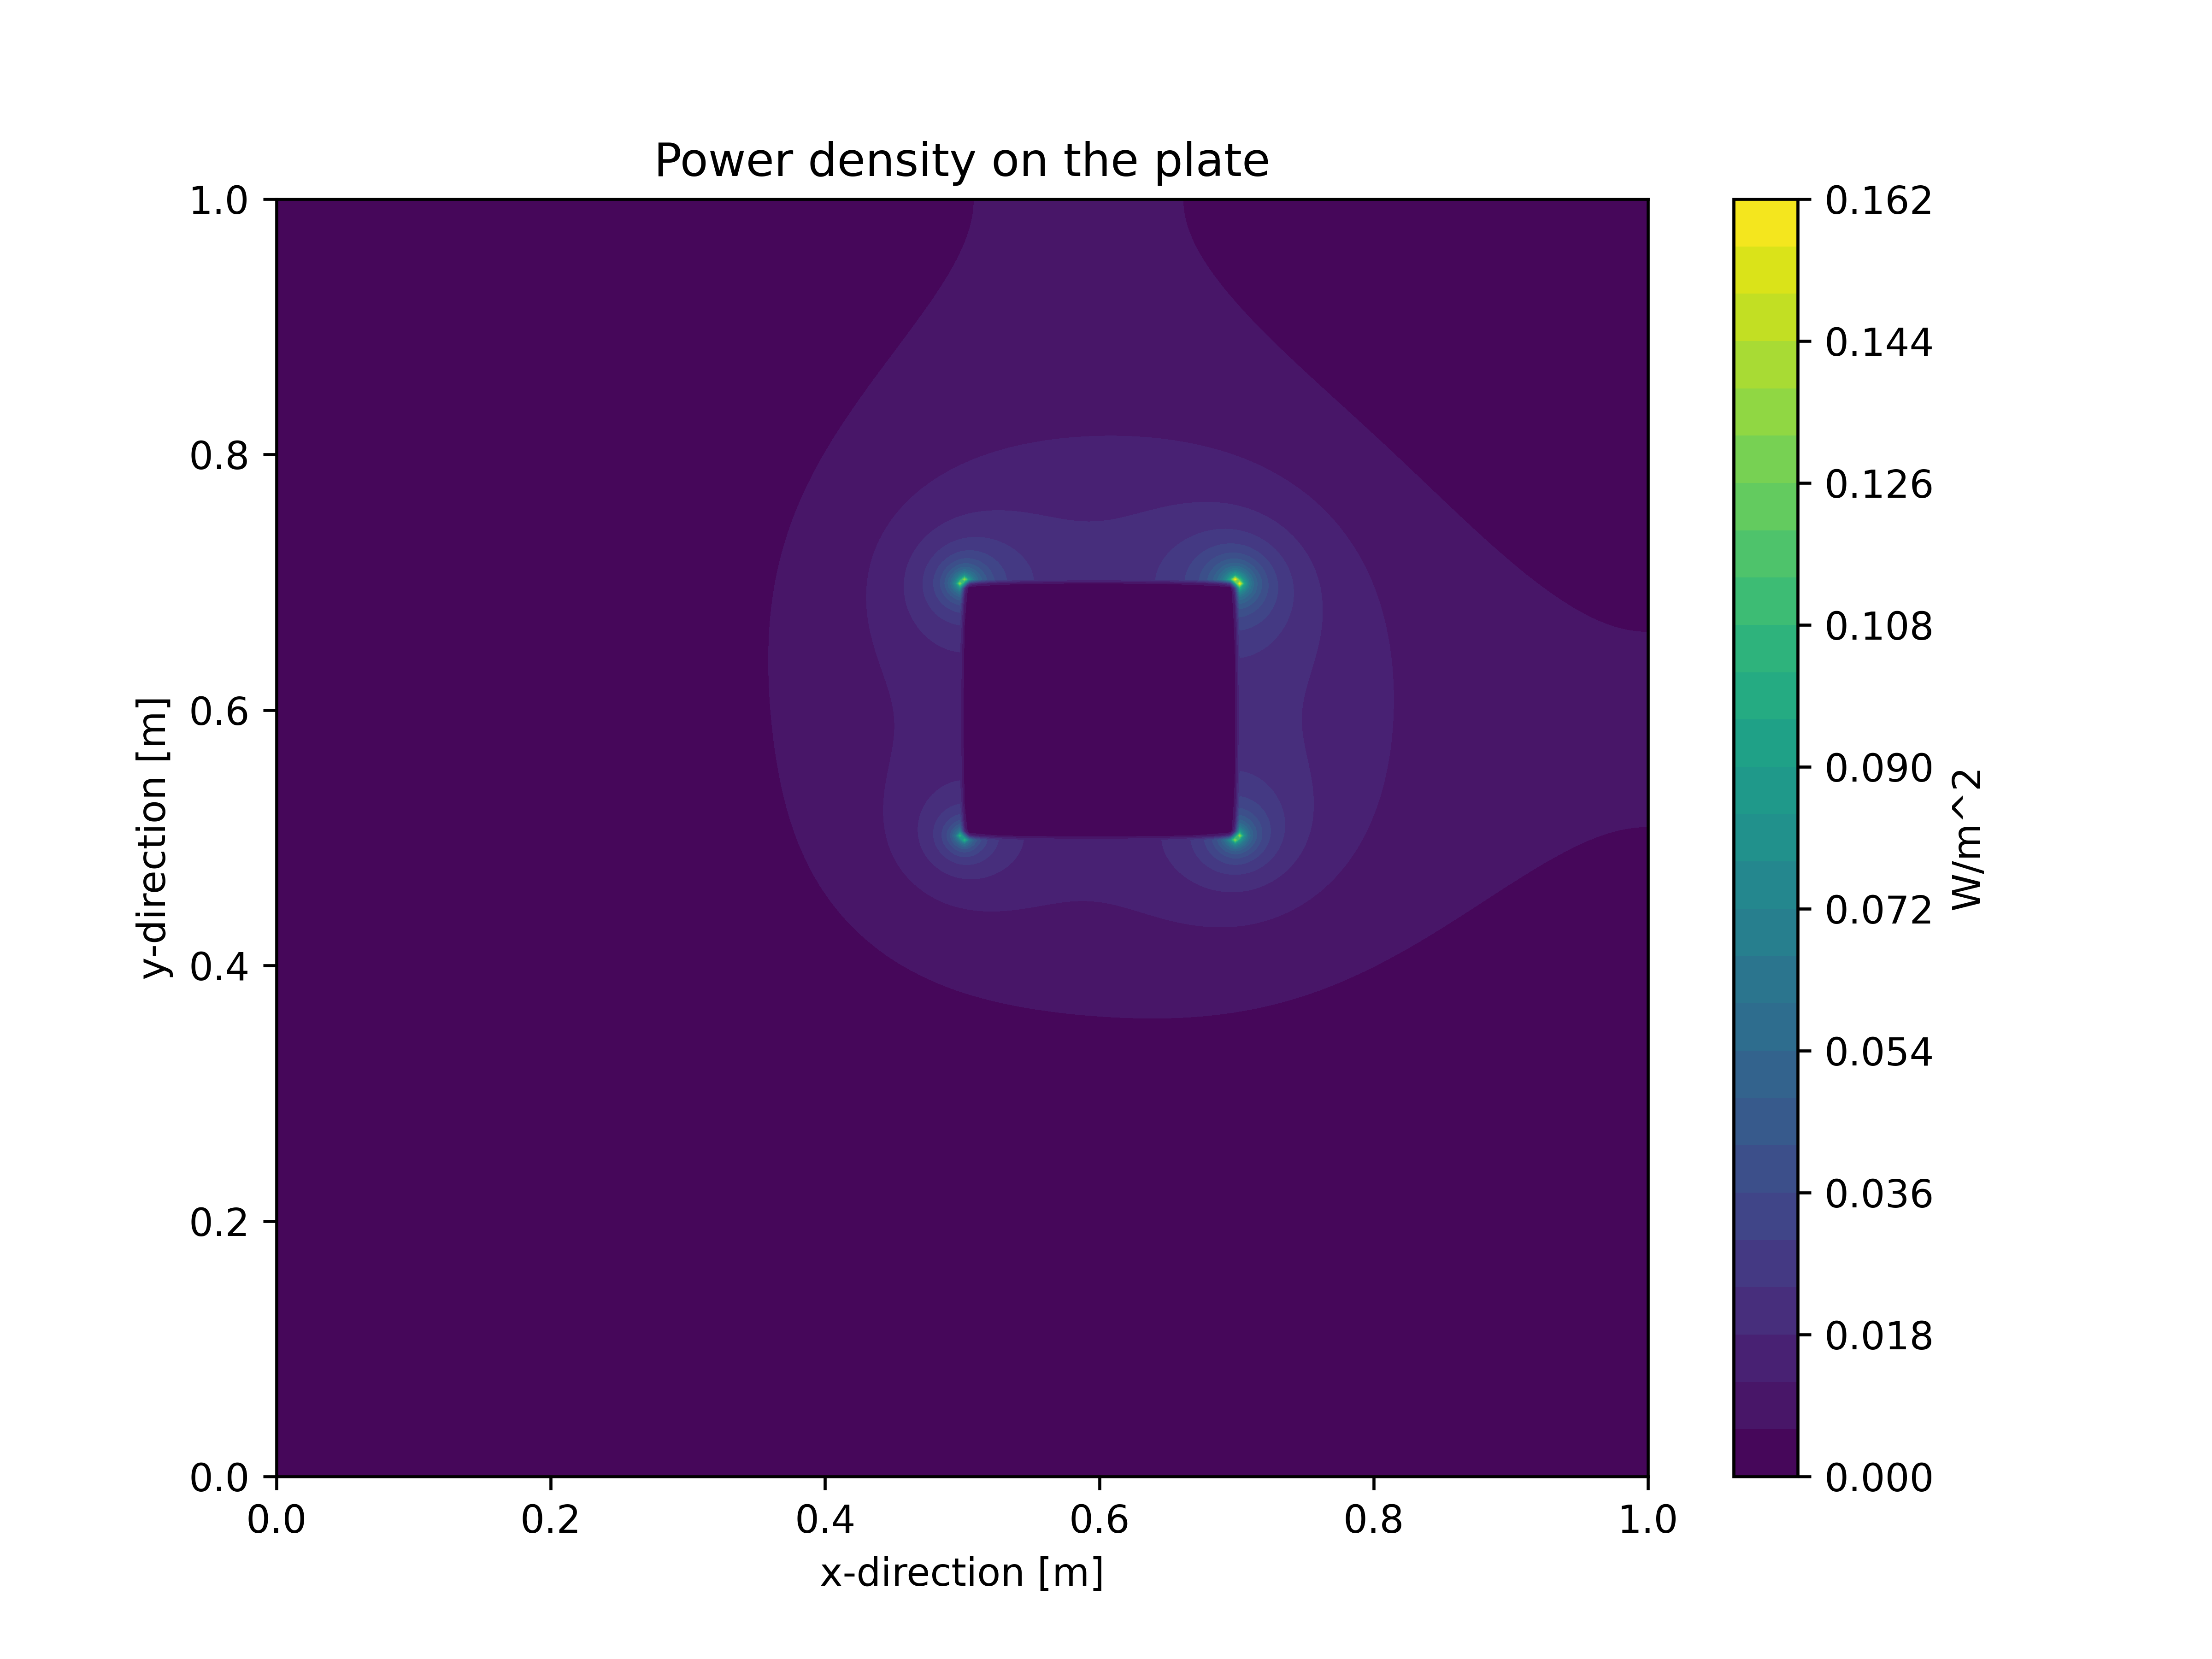
\includegraphics[width=0.99\textwidth]{papers/circuit/power_distribution.png}
	\caption{Power density 2d}
	\label{fig:power_2d}
\end{figure}
\begin{figure}[h]
	\centering
	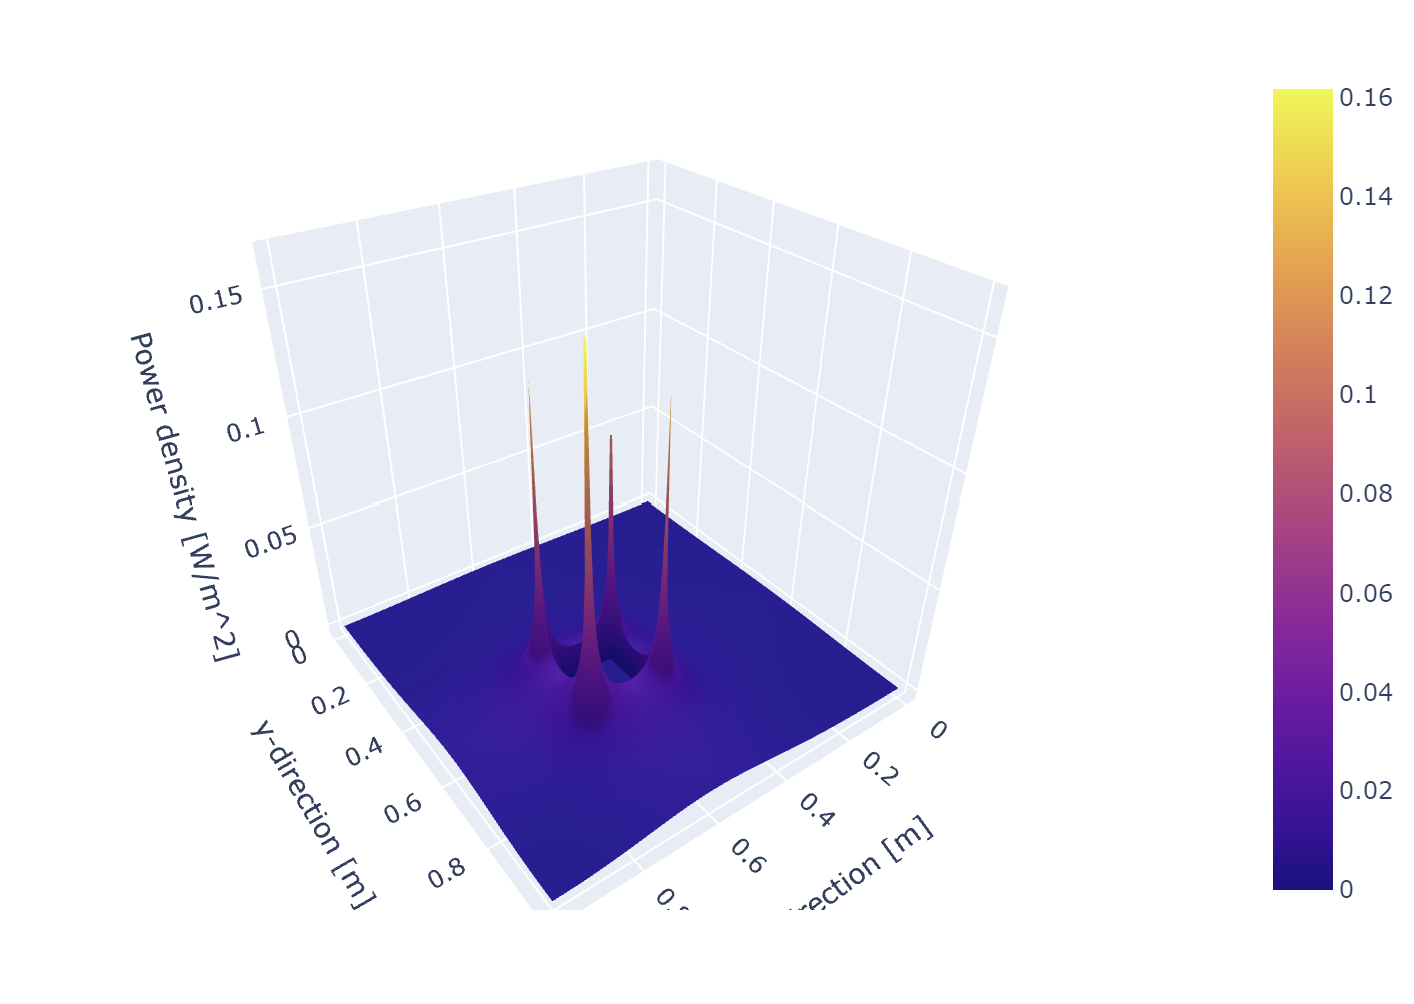
\includegraphics[width=0.99\textwidth]{papers/circuit/3d.png}
	\caption{Power density 3d}
	\label{fig:power_3d}
\end{figure}
Abbildung \ref{fig:power_3d} zeigt deutlich, dass die Leistungsdichte in den Ecken des quadratischen Potentials am höchsten ist. Dies ist der Hauptgrund, warum auf Leiterplatten oder PCBs normalerweise keine 90°-Kurven gezogen werden, sondern immer 45°-Kurven verwendet werden, um die Leistungsdichte bzw. Stromdichte in den Ecken zu minimieren.

%Als erstes importieren wir alle nötigen Bibliotheken in Python.
%\begin{lstlisting}[language=Python, caption=Python Librarys]
%"""
%Import the numpy library for numerical computations.
%"""
%import numpy as np
%"""
%Import the matplotlib.pyplot module from the matplotlib library for creating plots and visualizations.
%"""
%import matplotlib.pyplot as plt
%"""
%Import the numba library for just-in-time (JIT) compilation of Python code, which can significantly improve performance.
%"""
%import numba
%"""
%mpl_toolkits.mplot3d is a module from the matplotlib library that provides tools for creating 3D plots and visualizations.
%"""
%from mpl_toolkits.mplot3d import Axes3D
%"""
%matplotlib.cm is a module from the matplotlib library that provides a large set of colormaps for visualizing data in plots.
%"""
%from matplotlib import cm
%\end{lstlisting}
%Anschließend können wir die Berechnungen anhand von \autoref{circuit:discret_equation3} durchführen, wie es in \autoref{circuit:code1} gezeigt ist \footnote{Der Code wurde mithilfe von Copilot geschrieben}. 
%\begin{lstlisting}[language=Python, caption=Python Librarys, label=circuit:code1]
%def potential_block(x, y):
%	"""
%	Determine the potential value for a given (x, y) coordinate.
%	
%	Parameters:
%	x (float): The x-coordinate.
%	y (float): The y-coordinate.
%	
%	Returns:
%	float: The potential value for the given (x, y) coordinate.
%	"""
%	return np.select([(x>0.5)*(x<0.7)*(y>0.5)*(y<0.7),
%		(x<=0.5)+(x>=0.7)+(y<=0.5)+(y>=0.7)],
%		[1.,
%		0])
%@numba.jit("f8[:,:](f8[:,:], b1[:,:], i8)", nopython=True, nogil=True)
%def compute_potential(potential, fixed_bool, n_iter):
%	"""
%	Compute the potential
%	
%	Parameters:
%	- potential (numpy.ndarray): 2D array representing the potential.
%	- fixed_bool (numpy.ndarray): 2D boolean array indicating fixed points.
%	- n_iter (int): Number of iterations to perform.
%	
%	Returns:
%	- potential (numpy.ndarray): Updated potential after performing the iterations.
%	"""
%	length = len(potential[0])
%	for n in range(n_iter):
%		for i in range(1, length-1):
%			for j in range(1, length-1):
%				if not(fixed_bool[j][i]):
%					potential[j][i] = 1/4 * (potential[j+1][i] + potential[j-1][i] + potential[j][i+1] + potential[j][i-1])
%	return potential
%# define conductivity of the plate (siemens/m)
%sigma = 0.001
%# define size of plate in meters
%width=1
%height=1
%# define number of grid points in one direction
%n=300
%# define grid points
%x = np.linspace(0, width, n)
%y = np.linspace(0, height, n)
%# define potential at boundary points
%upper_y = 0 * x
%lower_y = 0 * x
%upper_x = 0 * y
%lower_x = 0 * y
%# create meshgrid for 2D potential xv are the x coordinates and yv are 
%# the y coordinates at each point, for example xv[0,0] is the x coordinate
%# of the first point and yv[0,0] is the y coordinate of the first point
%xv, yv = np.meshgrid(x, y)
%# create 2d array for potential
%potential = np.zeros((n,n))
%# set potential at boundary points
%potential[0,:]= lower_y
%potential[-1,:]= upper_y
%potential[:,0]= lower_x
%potential[:,-1]= upper_x
%# set potential inside the mesh to a predefined value one
%fixed = potential_block(xv,yv)
%fixed_bool = fixed!=0
%potential[fixed_bool] = fixed[fixed_bool]
%# calculate potential with numberical method and make n_iter iterations
%potential = compute_potential(potential,fixed_bool, n_iter=30000)
%# create a plot of the potential
%fig, ax = plt.subplots(1, 1, figsize=(8,6))
%clr_plot = ax.contourf(xv, yv, potential, 30)
%ax.set_xlabel('x-direction [m]')
%ax.set_ylabel('y-direction [m]')
%fig.colorbar(clr_plot, label='$V$')
%ax.set_title('Potential distribution in the plate')
%plt.show()
%\end{lstlisting}












%Wenn wir den Divergenzsatz/Gauscher Integralsatz (\autoref{circuit:gauscher_integralsatz}) anwenden und \autoref{circuit:current_density_6} verwenden, erhalten wir \autoref{circuit:leistung_gauscher_integralsatz}, da $\sigma$ ein skalar ist und die divergenz vom feld $\phi$ auch kann man den $\nabla$ operator ausklammern und hat die Gleichung dann genau in der Form dass man den satz von Gaus anwwenden kann.
%\begin{equation}
%	\oint_S \vec{F}_i \cdot \mathrm{d} \vec{S}=\int_V \nabla \cdot \vec{F}_i \mathrm{~d} V
%	\label{circuit:gauscher_integralsatz}
%\end{equation}
%
%
%
%
%
%
%
%\begin{equation}
%P=\int_V \nabla \cdot(\sigma \phi \nabla \phi) d V=\oint_S(\sigma \phi \nabla \phi) \cdot d \vec{S}
%\label{circuit:leistung_gauscher_integralsatz}
%\end{equation}
%
%Wenn die Leitfähigkeit im gesamten Volumen $V$ konstant ist, wird die Variation der Wärmeerzeugungsrate $P$ in $V$ gegeben durch \autoref{circuit:leistung_gauscher_integralsatz2}. Auf diese form der Gleichung kommt man wenn man das Kommutativgesetz und anschliessend die produkteregel  auf \autoref{circuit:leistung_gauscher_integralsatz} anwendet, wie es in \autoref{eq:produkteregel} gezeigt ist. Dabei ist zu beachten dass partielle Ableitungen für stetig differenzierbare funktionen vertauschbar sind ($\phi \nabla(\delta \phi) = \phi \delta(\nabla \phi)$).
%\begin{equation}
%\delta P=\sigma \oint_S(\delta \phi \nabla \phi) \cdot d \vec{S}+\sigma \oint_S(\phi \nabla(\delta \phi)) \cdot d \vec{S}
%\label{circuit:leistung_gauscher_integralsatz2}
%\end{equation}
%
%$$
%\delta[y(x)]=\bar{y}(x)-y(x)=\varepsilon\eta(x)
%$$
%
%
%\begin{equation}
%	\begin{aligned}
%		\delta P &=\sigma \cdot \delta \oint_S( \phi \nabla \phi) \cdot d \vec{S} = \sigma \cdot \oint_S \delta(\underbrace{\phi}_{u} \underbrace{\nabla \phi}_{v}) \cdot d \vec{S}\\
%		&= \sigma \cdot \oint_S \left(\underbrace{(\delta \phi)}_{u'} \cdot  \underbrace{(\nabla \phi)}_{v} + \underbrace{\phi}_{u} \cdot  \underbrace{\delta(\nabla \phi)}_{v'}\right)\cdot d \vec{S}
%	\end{aligned}
%	\label{eq:produkteregel}
%\end{equation}
%
%Nun haben wir die Gleichung gefunden und wir können die euler ostrogradsky differentialgleichung aus \cite{circuit:paper1} welche auch in \autoref{circuit:euler_lagransky} zu finden anwenden
%
%\begin{equation}
%	\textcolor{orange}{\frac{\partial F}{\partial z}(x, y, \phi, \frac{\partial \phi}{\partial x}, \frac{\partial \phi}{\partial y})}-\textcolor{brown}{\frac{\partial}{\partial x} \frac{\partial F}{\partial z_x}(x, y, \phi, \frac{\partial \phi}{\partial x}, \frac{\partial \phi}{\partial y})}-\textcolor{violet}{\frac{\partial}{\partial y} \frac{\partial F}{\partial z_y}(x, y, \phi, \frac{\partial \phi}{\partial x}, \frac{\partial \phi}{\partial y})}=0
%	\label{circuit:euler_lagransky}
%\end{equation}
%Machen wir das für den ersten teil der Gleichung und nehemen an das $\phi$ zwei dimensional ist und daher folgendes gilt $\phi=\phi(x,y)$
%\begin{equation}
%	\delta P=\sigma \oint_S(\delta \phi \nabla \phi) \cdot d \vec{S} \textcolor{gray}{+\sigma \oint_S(\phi \nabla(\delta \phi)) \cdot d \vec{S}}
%	\label{circuit:calc1}
%\end{equation}
%Wenn  wir die Formel nun anwenden kommen wir auf folgendes, da $\phi$ in der gleichung nur als ableitung vorkommt.
%\begin{equation}
%	\textcolor{orange}{\frac{\partial P}{\partial z}(x, y, \phi, \frac{\partial \phi}{\partial x}, \frac{\partial \phi}{\partial y})=0}
%\end{equation}
%\begin{equation}
%	\nabla=\frac{\partial}{\partial z} i+\frac{\partial}{\partial y} j+\frac{\partial}{\partial z} k
%	\label{circuit:nabla_operator}
%\end{equation}
%\begin{equation}
%	\textcolor{brown}{\frac{\partial}{\partial x}\frac{\partial P}{\partial \frac{\partial \phi}{\partial x}}(x, y, \phi, \frac{\partial \phi}{\partial x}, \frac{\partial \phi}{\partial y})
%	=\frac{\partial}{\partial x}\frac{\partial}{\partial \frac{\partial \phi}{\partial x}}\left(\delta \phi \left(\frac{\partial \phi}{\partial x} i+\frac{\partial \phi}{\partial y} j\right)\right)
%	=\frac{\partial}{\partial x}\left(\delta \phi \left(1+0\right)\right)}
%\end{equation}
%
%\begin{equation}
%	\textcolor{violet}{\frac{\partial}{\partial y}\frac{\partial P}{\partial \frac{\partial \phi}{\partial y}}(x, y, \phi, \frac{\partial \phi}{\partial x}, \frac{\partial \phi}{\partial y})
%	=\frac{\partial}{\partial y}\frac{\partial}{\partial \frac{\partial \phi}{\partial y}}\left(\delta \phi \left(\frac{\partial \phi}{\partial x} i+\frac{\partial \phi}{\partial y} j\right)\right)
%	=\frac{\partial}{\partial y}\left(\delta \phi \left(0+1\right)\right)}
%\end{equation}
%
%Setzen wir wieder alls zusammen bekommen wir folgendes:
%\begin{equation}
%	\textcolor{orange}{0}-\textcolor{brown}{\frac{\partial}{\partial x}\left(\delta \phi \left(1+0\right)\right)} - \textcolor{violet}{\frac{\partial}{\partial y}\left(\delta \phi \left(0+1\right)\right)}=0
%\end{equation}
%
%\begin{equation}
%	\Delta \phi(x,y)=\frac{\delta^2\phi}{\delta x^2}+\frac{\delta^2\phi}{\delta y^2}=0
%\end{equation}
%\begin{equation}
%	\Delta h(x)=0
%\end{equation}
%
%
%
%Aus \autoref{circuit:leistung_gauscher_integralsatz2} geht hervor, dass wenn Variationen im Fluss, $\delta \phi$, an der Grenze von $V$ verschwinden, dann ist $P$ stationär, d.h. $\delta P=0$. Daher werden elektrische Ströme in der Region verteilt, mit einer angelegten Spannung an ihrer Grenze,
%
%
%\begin{figure}
%	\centering
%	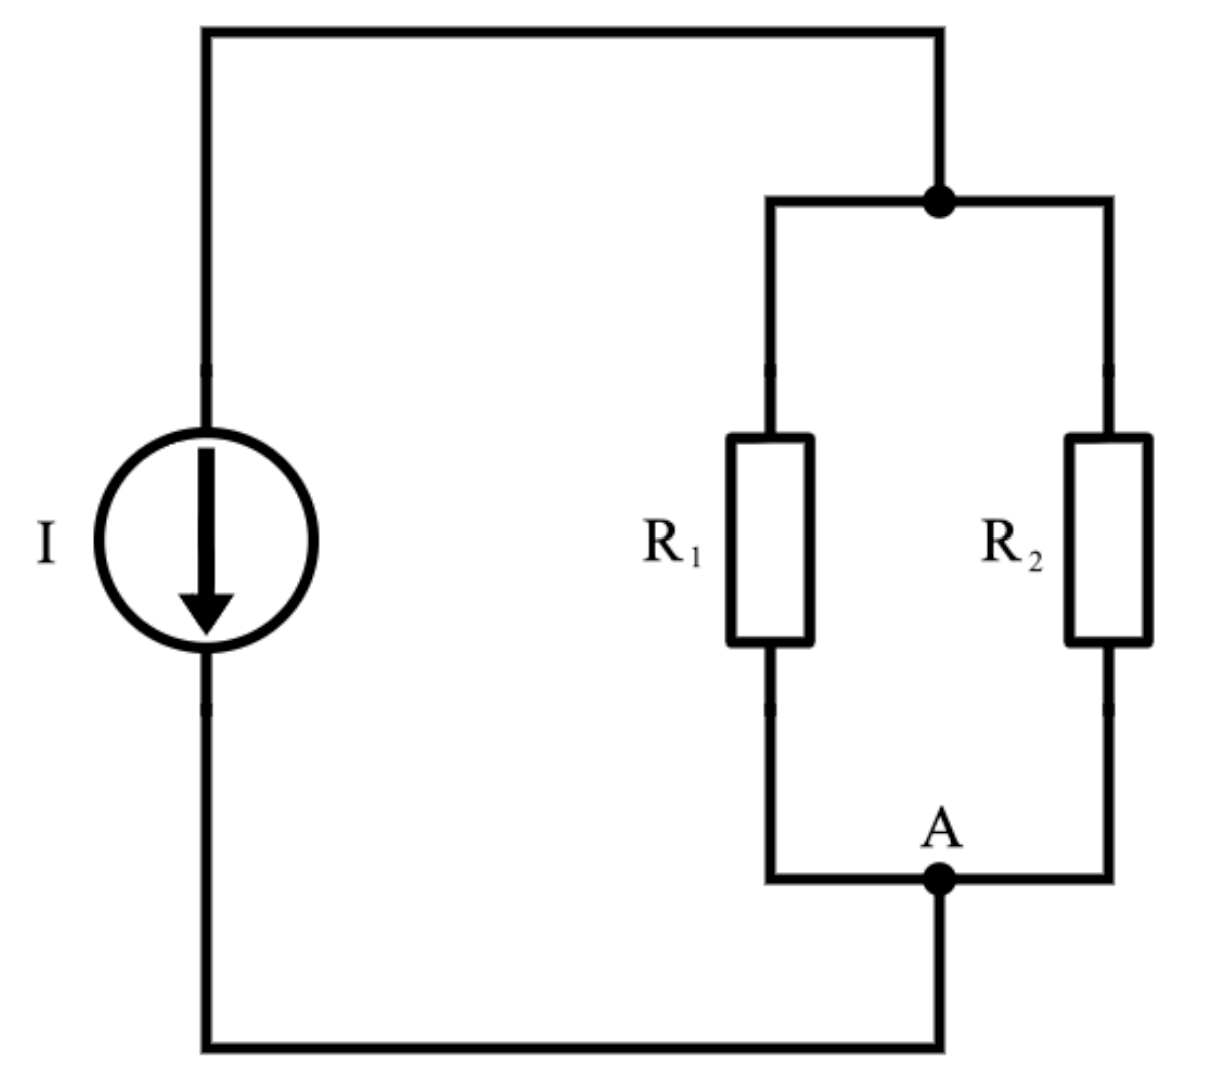
\includegraphics[width=0.6\textwidth]{papers/circuit/images/image_01.png}
%	\caption{Parrallelschaltung von zwei Wiederständen \cite{circuit:bibtex}
%	\label{papers:circuit:images:parallelschaltung_strom}}
%\end{figure}




%https://www.youtube.com/watch?v=VCHFCXgYdvY
